\documentclass[12pt,a4paper]{article}
\usepackage{packages_for_thesis}
\usepackage{commands}
\usepackage{enumerate}

\addbibresource{complexnet.bib}

\setlength{\headheight}{14.49998pt}

\hypersetup{
    colorlinks=true,     
    urlcolor=blue}

\newtheorem{theorem}{Theorem} % Defines the "theorem" environment
%%%%%%%%%%%%%%%%%%%%%%%%%%%%%%%%%%%%%%%%BEGIN DOCUMENT

\begin{document}

\begin{titlepage}
%
%
\begin{center}
{{\Large{\textsc{Alma Mater Studiorum $\cdot$ Universit\`a di Bologna}}}} 
\rule[0.1cm]{15.8cm}{0.1mm}
\rule[0.5cm]{15.8cm}{0.6mm}
\\\vspace{3mm}

{\small{\bf Complex Networks \\ \vspace{2mm}
Lorenzo Fabbri}}

\end{center}

%I want the title to be vertically centered
\topskip0pt  
\vspace*{\fill}

\begin{center}
{\LARGE{\bf Discrete Ricci Flow applied to Facebook Ego Network}\\
}\end{center}

\vspace*{\fill}

\vspace{50mm} \par \noindent

\begin{center}
%
Academic Year \textcolor{black}{2024/2025}
\end{center}

\end{titlepage}

\selectlanguage{English}

\begin{abstract}
    \noindent This project uses Ricci Flow as a geometric approach to detect community structures in networks. It applies Ollivier-Ricci curvature to adjust the weights of edges in a graph, iterating the process to shrink intra-community edges and stretch inter-community edges. Planar graphs with different community structures are used as datasets, with the goal of identifying pre-labelled communities using the Ricci Flow method. 

\end{abstract}

\vspace{2cm}

\tableofcontents
\addtocontents{toc}{\protect\thispagestyle{empty}}
\thispagestyle{empty}

\newpage 
\setcounter{secnumdepth}{-1}

\mainmatter

\setcounter{secnumdepth}{2}
\pagestyle{fancy}
\renewcommand{\sectionmark}[1]{\markboth{#1}{#1}}
\fancyhead[R]{}
\fancyhead[L]{\thesection \MakeUppercase{\textit{\ --\ \leftmark}}}

\section{Introduction}
The study of networks has gained considerable attention in various fields, ranging from sociology to biology, and beyond. One of the central problems in network science is community detection, where the objective is to identify groups of nodes (communities) that are more densely connected internally than with the rest of the network. Traditional methods for community detection often rely on statistical or combinatorial approaches. However, recent developments in geometric methods have introduced new ways to approach this problem by leveraging concepts from differential geometry \cite{communitydetectionnetworksricci}.

A powerful geometric tool, the Ricci Flow, originally developed in the context of smooth Riemannian manifolds, can be adapted to discrete network structures. In its original formulation, the Ricci Flow evolves the metric of a manifold according to the curvature (represented by Ricci tensor), leading to a smoothing process over time. Ollivier-Ricci curvature, a discretization of Ricci curvature for graphs, provides a framework to extend this idea to networks, where the "curvature" of edges encodes structural information about node connectivity. Specifically, positive curvature tends to shrink intra-community edges, while negative curvature expands inter-community edges \cite{communitydetectionnetworksricci}.

In this project, we explore the application of Ricci Flow in community detection by focusing on planar graphs, i.e. graphs that can be drawn on a plane without any edges crossing each other. By applying Ollivier-Ricci curvature to this network, we aim to assign and iteratively modify the curvature of edges, enhancing intra-community cohesion while stretching inter-community connections. Starting from graphs in which all the edges have weights set to 1, the flow will introduce weight diversity based on the topological characteristics of the graph, allowing observation of the natural curvature-driven "deformation" of the network.

The results will be compared to the predefined community labels, allowing for a direct comparison between the detected communities and the actual community structures. 

The developed code can be accessed in the corresponding GitHub repository: \textit{\href{https://github.com/fabbri-lorenzo/RicciFlowNetwork}{RicciFlowNetwork}}.
\newpage

\section{Ricci Flow Method}
Given a manifold $M$, a \textit{Ricci Flow} is a smooth family $g(t)$, with $ t \in [0,T)$, of Riemannian metrics satisfying the evolution equation

\begin{equation}\label{eq1}
    \partial_t g(t) = -2 Ric_{g(t)}
\end{equation}
where $Ric_{g(t)}$ is the Ricci tensor for the metric $g(t)$, i.e. the contraction of the Riemann tensor obtained with $g(t)$; in components $Ric_{g(t)}^{ij} \equiv g_{kl}(t)R^{iklj}$ \cite{recentdevelopmentsricciflows}.

The metric is deformed in a way which smooths out its irregularities, like in a heat diffusion process. Indeed, using harmonic local coordinates, the Ricci tensor approximates the Laplacian\footnote{Actually the operator $\triangle$ in Equation \hyperref[eq2]{2} is the Laplace-Beltrami operator, a generalization of the Laplace operator to functions defined on Riemannian and pseudo-Riemannian manifolds.} of the metric up to lower-order terms in derivatives of the metric tensor:
\begin{equation}\label{eq2}
    Ric_{g} = -\frac{1}{2}\triangle g + \textit{lower-order terms}
\end{equation}
which plugged into Equation \hyperref[eq1]{1} results in a nonlinear heat equation \cite{theRicciFlowAnIntroduction}.

By viewing a network as a discrete analogue of a 3-manifold, we can interpret the process of community detection as a geometric decomposition analogous to how Ricci Flow decomposes a 3-manifold into distinct geometric regions. Each community in the network represents a cohesive region of the network, much like a geometric region in a manifold. 
Inter-community edges are analogous to the boundaries between geometric regions in the manifold while intra-community edges represent connections within a homogeneous geometric region.


\subsection{Ollivier's Ricci Curvature}

Ollivier's Ricci curvature is a discrete adaptation of the classical Ricci curvature defined for smooth manifolds, tailored for graph structures. In a network, nodes represent points, and edges between them denote "distances" or connections. Rather than relying on continuous geometry, Ollivier's Ricci curvature measures how well-connected neighboring nodes are by comparing the distances between their neighborhoods.

In a graph, each node $x$ has a set of neighboring nodes, and we assign a probability distribution over this set, denoted as $m_x$. This distribution can be thought of as how much "mass" each neighbor carries. For example, the nodes $x$ and $y$ in Figure \hyperref[fig1]{1} each have three neighbors, and the respective probability distributions over their neighborhoods are denoted as $m_x$ and $m_y$.

\begin{figure}[ht] \label{fig1}
    \centering
    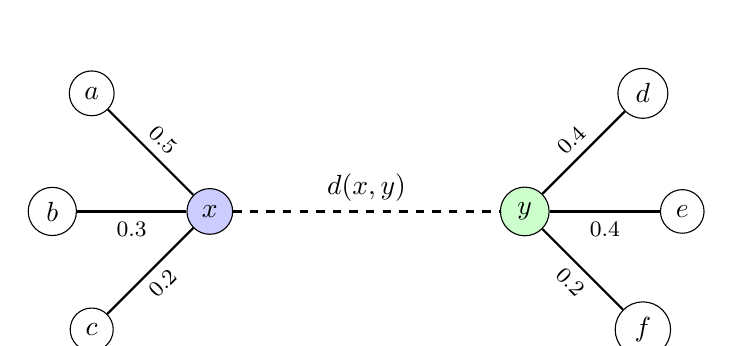
\begin{tikzpicture}
        % Nodes for x and its neighbors
        \node[draw, circle, fill=blue!20] (x) at (0, 0) {$x$};
        \node[draw, circle] (a) at (-1.5, 1.5) {$a$};
        \node[draw, circle] (b) at (-2, 0) {$b$};
        \node[draw, circle] (c) at (-1.5, -1.5) {$c$};
        
        % Nodes for y and its neighbors
        \node[draw, circle, fill=green!20] (y) at (4, 0) {$y$};
        \node[draw, circle] (d) at (5.5, 1.5) {$d$};
        \node[draw, circle] (e) at (6, 0) {$e$};
        \node[draw, circle] (f) at (5.5, -1.5) {$f$};
        
        % Edges connecting x and its neighbors
        \draw[thick] (x) -- (a) node[midway, above, sloped] {\footnotesize 0.5};
        \draw[thick] (x) -- (b) node[midway, below] {\footnotesize 0.3};
        \draw[thick] (x) -- (c) node[midway, below, sloped] {\footnotesize 0.2};
        
        % Edges connecting y and its neighbors
        \draw[thick] (y) -- (d) node[midway, above, sloped] {\footnotesize 0.4};
        \draw[thick] (y) -- (e) node[midway, below] {\footnotesize 0.4};
        \draw[thick] (y) -- (f) node[midway, below, sloped] {\footnotesize 0.2};
        
        % Edge between x and y
        \draw[thick, dashed] (x) -- (y) node[midway, above] {$d(x, y)$};
    \end{tikzpicture}
    \caption{Nodes $x$ and $y$ with their respective neighborhoods and probability distributions. The weights on the edges represent the probability distribution $m_x$ for node $x$'s neighbors and $m_y$ for node $y$'s neighbors.}
\end{figure}



Formally, the Ollivier-Ricci curvature $\kappa(x, y)$ between two connected nodes $x$ and $y$ is defined using the \textit{earthmover's distance}, also known as the \textit{Wasserstein distance}, between probability distributions on the neighborhoods of $x$ and $y$:
\begin{equation}\label{eq3}
    \kappa(x, y) = 1 - \frac{W_1(m_x, m_y)}{d(x, y)}
\end{equation}
where
\begin{itemize}
    \item $d(x, y)$ is the shortest path distance between nodes $x$ and $y$.
    \item $W_1(m_x, m_y)$ is the Wasserstein-1 distance between the probability distributions of neighboring nodes around $x$ and $y$:
    \begin{equation}
        W_1(m_x, m_y) = \textit{inf} \left\{ \left. \int\limits_{X \times Y} d(x,y) d\gamma(x,y) \right| \gamma \in \Gamma(m_x, m_y)  \right\}
    \end{equation}
    with $\gamma$ being a probability measure on $X \times Y$ (the probability spaces of the neighboring nodes around $x$ and $y$) and $\Gamma(m_x, m_y)$ indicating the collection of all possible transportation plans.
\end{itemize}

This curvature provides a natural way to quantify the coupling between two neighborhoods. High positive curvature implies that the neighborhoods of $x$ and $y$ are tightly connected, whereas negative curvature indicates sparse or loosely connected regions \cite{communitydetectionnetworksricci}.

Edges with high positive curvature tend to represent intra-community connections, while edges with low or negative curvature correspond to inter-community links. This distinction allows us to leverage geometric intuition for community detection, adjusting edge weights based on their curvature values.




\subsection{The Discrete Ricci Flow Algorithm}
The discrete Ricci flow algorithm modifies the concept of Ricci Flow to suit network structures by iteratively updating the weights of the edges according to their curvature values. The steps of the algorithm are as follows:

\begin{enumerate}
    \item \textbf{Initialization}: Begin with a graph $G(V, E)$, where $V$ is the set of vertices and $E$ is the set of edges. Each edge $(x, y) \in E$ is assigned an initial weight, which can be based on the shortest path distance between nodes $x$ and $y$, or on a predefined edge weight.
    
    \item \textbf{Curvature Computation}: For each edge $(x, y)$, compute the Ollivier-Ricci curvature $\kappa(x, y)$. The Wasserstein distance here is defined as the minimum total weighted travel distance to move $m_x$ to $m_y$, i.e.
    \begin{equation}
        W(m_x,m_y) =  \textit{inf} \left\{ \sum\limits_{u,v\in V} A(u,v) d(u,v)  \right\}
    \end{equation}
    where $A(u,v)$ is a map $V\times V \rightarrow [0,1]$ called \textit{discrete transport plan}. It corresponds to the amount of mass moved from vertex $u \in V_x$ (a neighbor of $x$) to vertex $v \in V_y$ (a neighbor of $y$). The transport plan satisfies $\sum_{v \in V} A(u,v) = m_x(u)$ and $\sum_{u \in V} A(u, v) = m_y(v)$, where $m_x (u)$ and $m_y(v)$ are the probability distributions on the neighborhoods of $x$ and $y$ respectively. These conditions ensure that the total mass leaving node $x$ matches the distribution $m_x$, and the total mass arriving at node $y$ matches $m_y$.
    \item \textbf{Edge Weight Update}: Modify the weights of the edges based on their curvature values. If $\kappa(x, y)$ is positive, reduce the edge weight, simulating a contraction of intra-community edges. Conversely, if $\kappa(x, y)$ is negative, increase the edge weight, stretching inter-community edges. The updated weight $w'(x, y)$ is given by:
    \begin{equation}\label{eq4}
    w'(x, y) = w(x, y) \times (1 - \alpha \cdot \kappa(x, y))
    \end{equation}
    where $\alpha$ is a step size parameter controlling the rate of change.
    
    \item \textbf{Iteration}: Repeat the process of computing curvature and updating edge weights for a specified number of iterations or until convergence is achieved. Over time, intra-community edges shrink (strengthen) while inter-community edges stretch (weaken), causing communities to become more distinct.

    \item \textbf{Surgery Process}: Remove edges that contribute to singularities. Edges with a curvature value below a certain threshold, typically set $\approx -0.1$, are pruned. It is worth mentioning that there are other techniques to modify the graph structure to deal with problematic regions, effectively 'surgically' altering the graph to maintain the flow's stability. Common ones are edge contraction (i.e. reducing the weight of edges that are causing high curvature) and node splitting (i.e. dividing a single node into multiple nodes while redistributing the connected edges among them).
    

    \item \textbf{Community detection}: After the edge weights have been updated through the Ricci Flow iterations, we apply the Louvain method for community detection, which returns a partition of the network based on the modified edge weights from the Ricci Flow process, where each node is assigned to a community.  
\end{enumerate}



\subsection{Convergence Criteria and Stopping Conditions} \label{sec2.3}
The theoretical foundation of the discrete Ricci Flow method for community detection is supported by several key results, one of the most important being the convergence guarantees provided by Theorem 4.1 from \cite{communitydetectionnetworksricci}.

\begin{theorem}[Theorem 4.1, \cite{communitydetectionnetworksricci}] \label{th1}
The Ricci flow associated with the Ollivier $K_0$-Ricci curvature \footnote{$K_0$-Ricci curvature is a modification of Ollivier-Ricci curvature which incorporates a parameter $K_0$ in order to adjust the curvature calculation; emphasizing certain aspects of community structure.} detects the community structure on $G(a, b)$ if $a > b \geq 2$. Specifically, the algorithm asymptotically shrinks the weights of intra-community edges faster than the weights of inter-community edges. %This process effectively partitions the graph $G(a, b)$ into distinct communities.
\end{theorem}

Theorem \hyperref[th1]{1} guarantees the convergence of the discrete Ricci Flow algorithm, meaning that after a finite number of iterations, the edge weights stabilize and no further significant changes occur. This convergence ensures that the community structure revealed by the Ricci Flow process is robust and does not depend on further iterations.

While Ricci Flow has inherent convergence properties that can lead to well-separated communities, some practical stopping conditions will often be required for implementation:

\begin{enumerate}
    \item \textbf{Change in Edge Weights}: 
    Monitor the change in edge weights between iterations. Convergence is achieved when the change falls below a predefined threshold $\epsilon$, indicating that the algorithm has stabilized:
    \[
    \max_{(x, y) \in E} |w_{\text{new}}(x, y) - w_{\text{old}}(x, y)| < \epsilon
    \]
    
    \item \textbf{Community Structure Stability}: 
    Validate the stability of the detected community structure across iterations. Ensure that identified communities remain consistent and meaningful by assessing their internal cohesion and external separation.
    
    \item \textbf{Maximum Iterations}: 
    Define a maximum number of iterations $N_{\text{max}}$ to prevent excessive computation and to facilitate early stopping if convergence is not achieved within this limit:
    \[
    \text{If } k > N_{\text{max}}, \text{ stop algorithm}
    \]
\end{enumerate}



\newpage


\section{Implementation in a Toy Model}
Before implementing the method discussed above to planar graphs, we first investigate Ricci curvature flow on three types of simple graphs: a stochastic block model (SBM) graph, a Barbell graph, and a Caveman graph. Each graph type exhibits distinct structural properties, facilitating a comprehensive exploration of Ricci flow dynamics.

\subsection{\textit{GraphRicciCurvature} Library}
In addition to the main library for networks, \textit{Networkx}, the developed code relies on the \textit{GraphRicciCurvature} library, which provides efficient algorithms for calculating the Ollivier-Ricci curvature on graphs.

Key features of the \textit{GraphRicciCurvature} library include:

\begin{itemize}
    \item \textbf{OllivierRicci Class}: This class is initialized with the graph and a parameter \texttt{alpha}, which controls the curvature's sensitivity to edge weights. Smaller alpha values (closer to 0) are often used when one focuses on local community detection, small subgraphs, or clusters. Larger alpha values (closer to 1) are used when the interest is in the global structure of the graph, such as long-range connections and global topology.
    
    \item \textbf{Curvature Computation}: The method \texttt{compute\_ricci\_curvature()} calculates the Ricci curvature for all edges in the graph.
    
    \item \textbf{Edge Curvature Assignment}: After computing the curvatures, the edge attributes of the original graph are updated with the curvature values calculated by the \texttt{OllivierRicci} instance. 
\end{itemize}



\subsection{Results}

The Ricci Flow method was tested on three different types of graphs to evaluate its functionalities and performance. Each graph has distinct structural properties, making them ideal candidates for assessing the method’s ability to identify both densely connected intra-community edges and sparser inter-community edges. For each graph type the Ricci Flow process has been simulated using 15 iterations and an alpha of 0.5. The results are summarized below. 

\textbf{Stochastic Block Model (SBM) graph}: This graph is specifically designed to simulate community structures with predefined groups. Nodes within the same group are more likely to connect, while connections between groups are less frequent. We created an SBM graph with two communities of 50 nodes each, where the intra-community edge probability was set high to ensure clear separation between the communities. The Ricci Flow method (with threshold for surgery set to -0.05) successfully identified the two distinct communities, as illustrated in Figure \hyperref[fig2]{2}.

\textbf{Barbell graph}: The barbell graph consists of two complete graphs (dense communities) connected by a path (sparse inter-community links). It is an excellent test case for methods that detect clear community boundaries with sparse connections between them. In our experiments, we used a barbell graph with two communities of 20 nodes each, connected by a 5-node path. The method  (with threshold for surgery set to -0.1) correctly detected the two communities, with the inter-community path clearly stretched due to the low curvature, as seen in Figure \hyperref[fig3]{3}.

\textbf{Caveman graph}: A caveman graph is another community-like structure where several cliques (complete subgraphs) are loosely connected. This type of graph is useful for testing models aimed at detecting clique-based communities. We tested the method on a caveman graph with 5 cliques, each consisting of 10 nodes. The method (with threshold for surgery set to 0) successfully separated the cliques, identifying each as a distinct community, as shown in Figure \hyperref[fig4]{4}.

Across all three graph types, the developed Ricci Flow-based method behaved as expected, demonstrating its capability to detect both dense and sparse community structures. The method shrank intra-community edges and stretched inter-community edges, which aligns with the behavior predicted by the underlying theory of Ollivier-Ricci curvature. The results from the tests on the SBM graph, Barbell graph, and Caveman graph are displayed in Figures \hyperref[fig2]{2}, \hyperref[fig3]{3}, and \hyperref[fig4]{4} respectively; edges with different colours belong to different communities. 

Additional results and details, such as plots of the networks after Ricci Flow and after surgery,  can be found on the project's GitHub page.


\begin{figure}[h]
    \centering
    \begin{subfigure}[b]{0.45\textwidth}
        \centering
        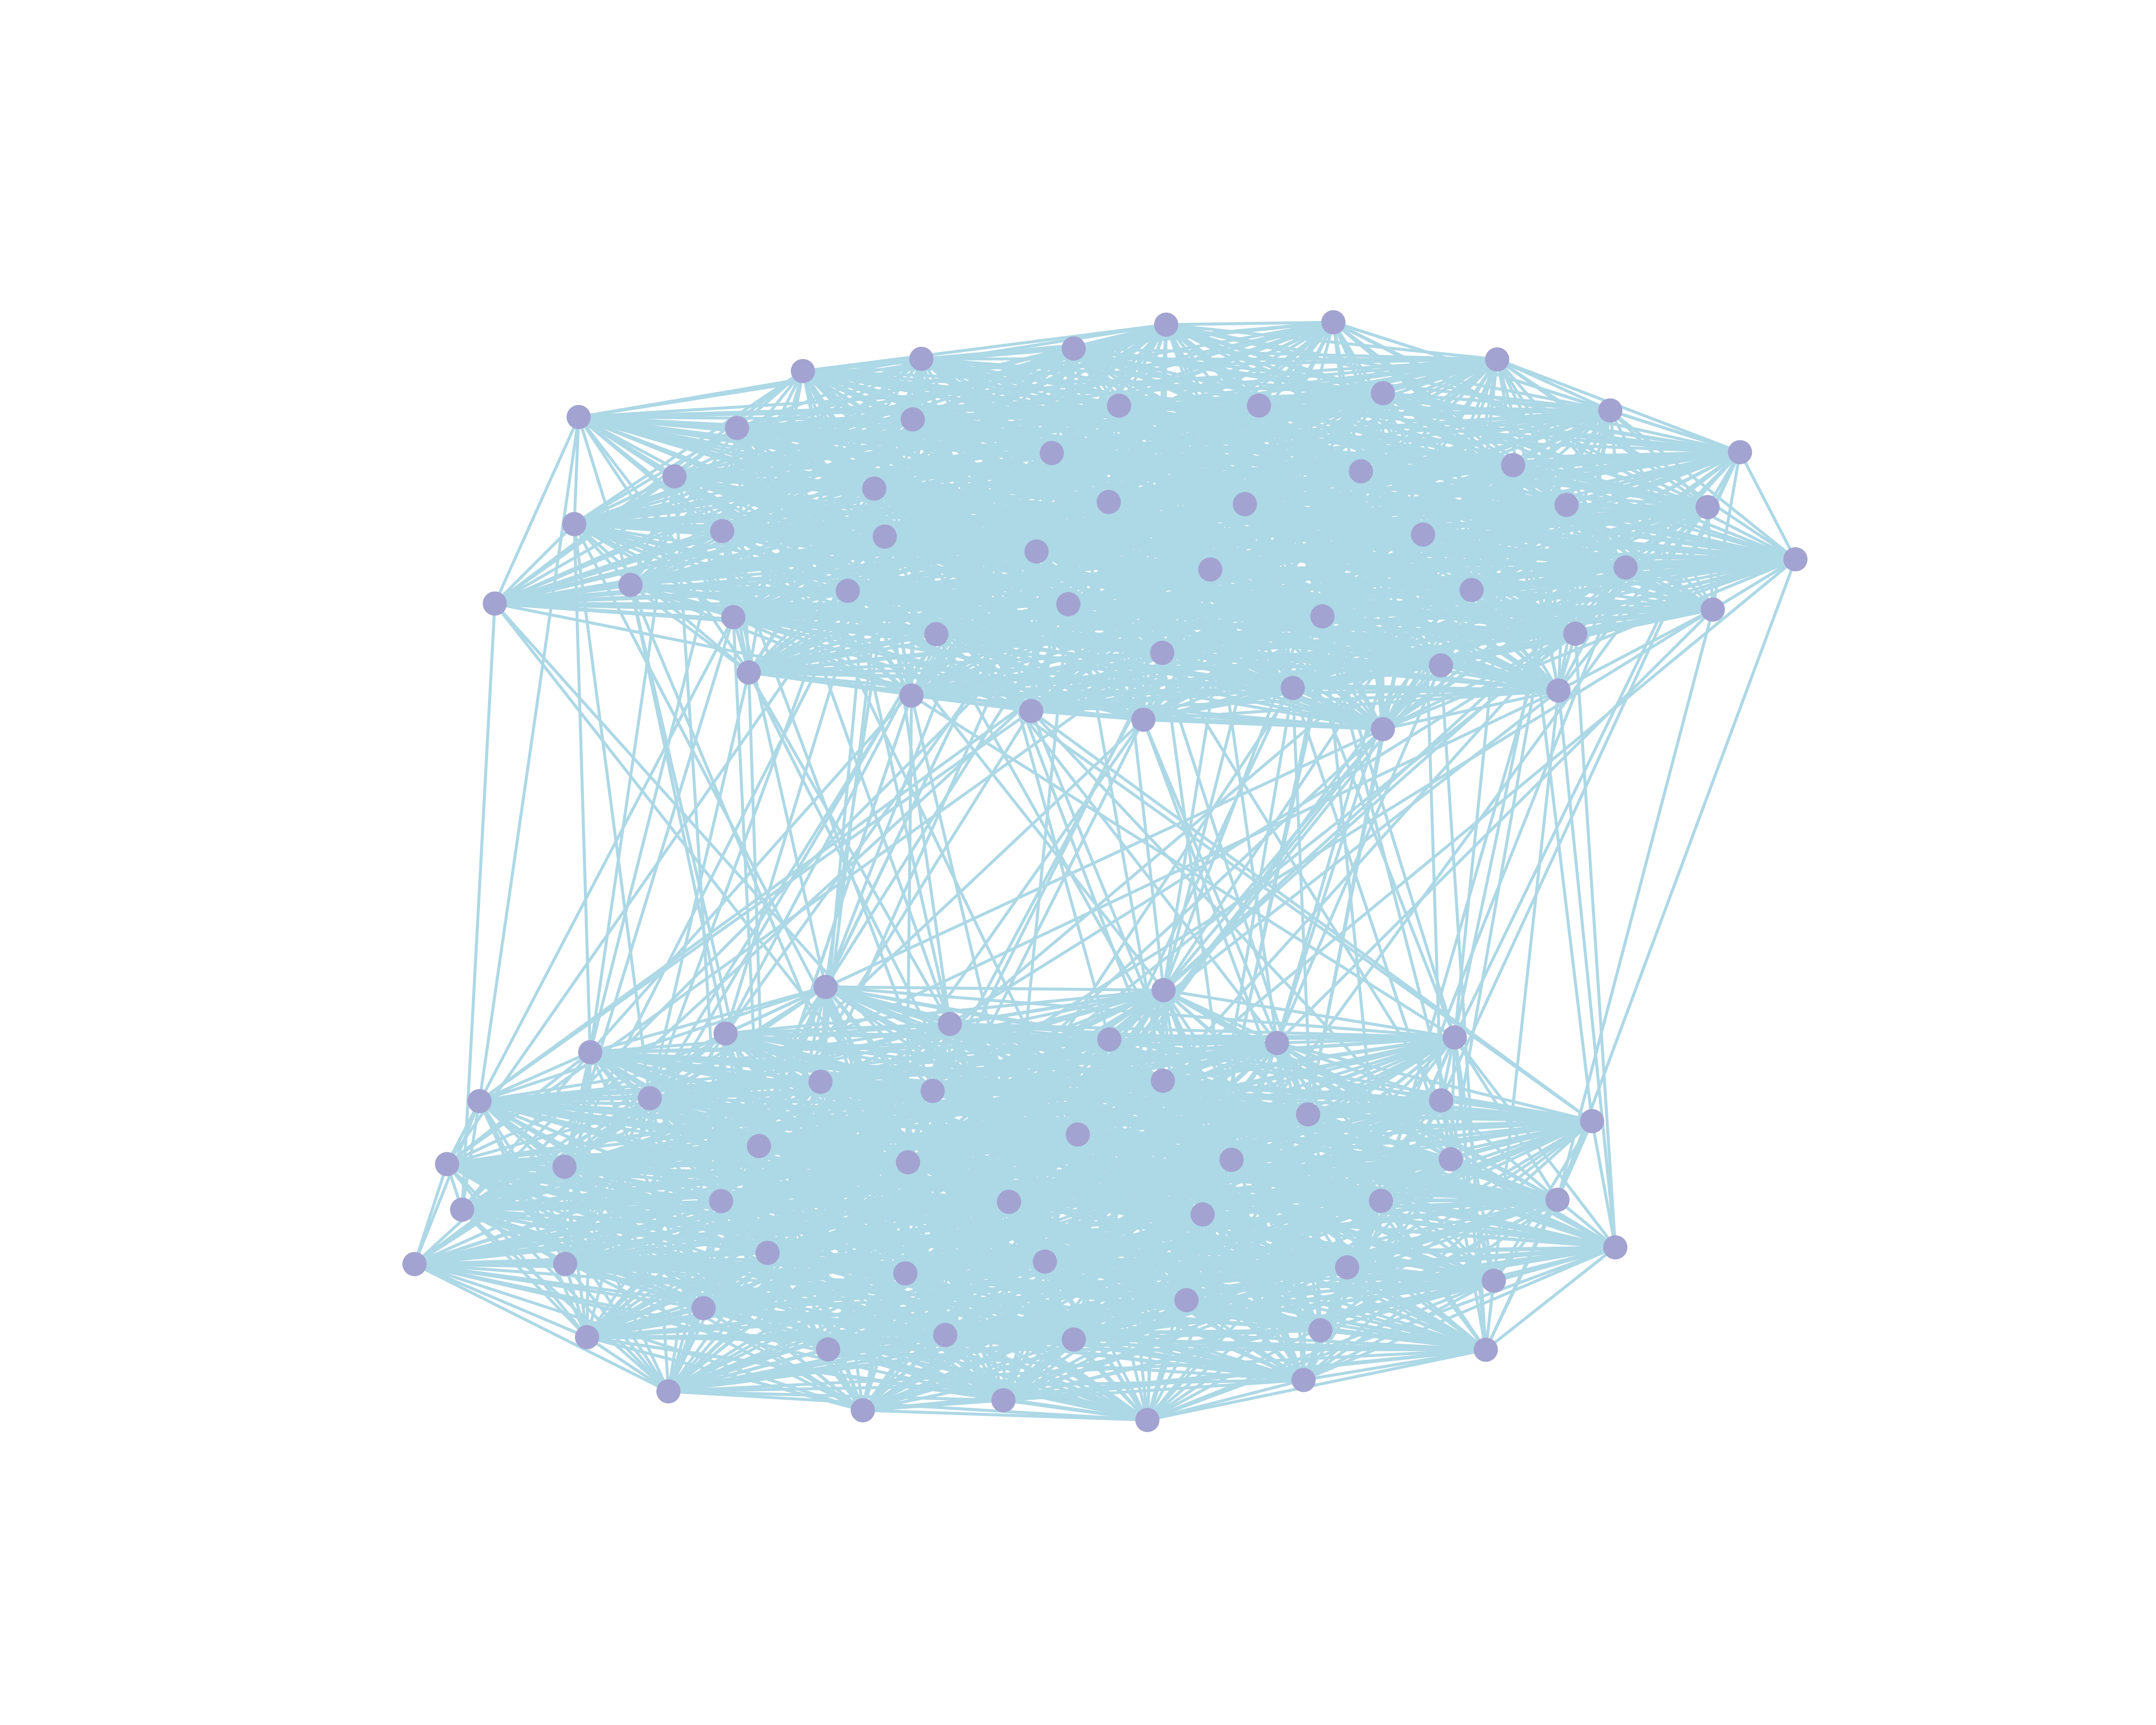
\includegraphics[width=\textwidth]{ToyModelResults/SBM_results/BeforeRicciFlow.png}
        \caption{Initial SBM graph}
        \label{fig:sbm_initial}
    \end{subfigure}
    \hfill
    \begin{subfigure}[b]{0.45\textwidth}
        \centering
        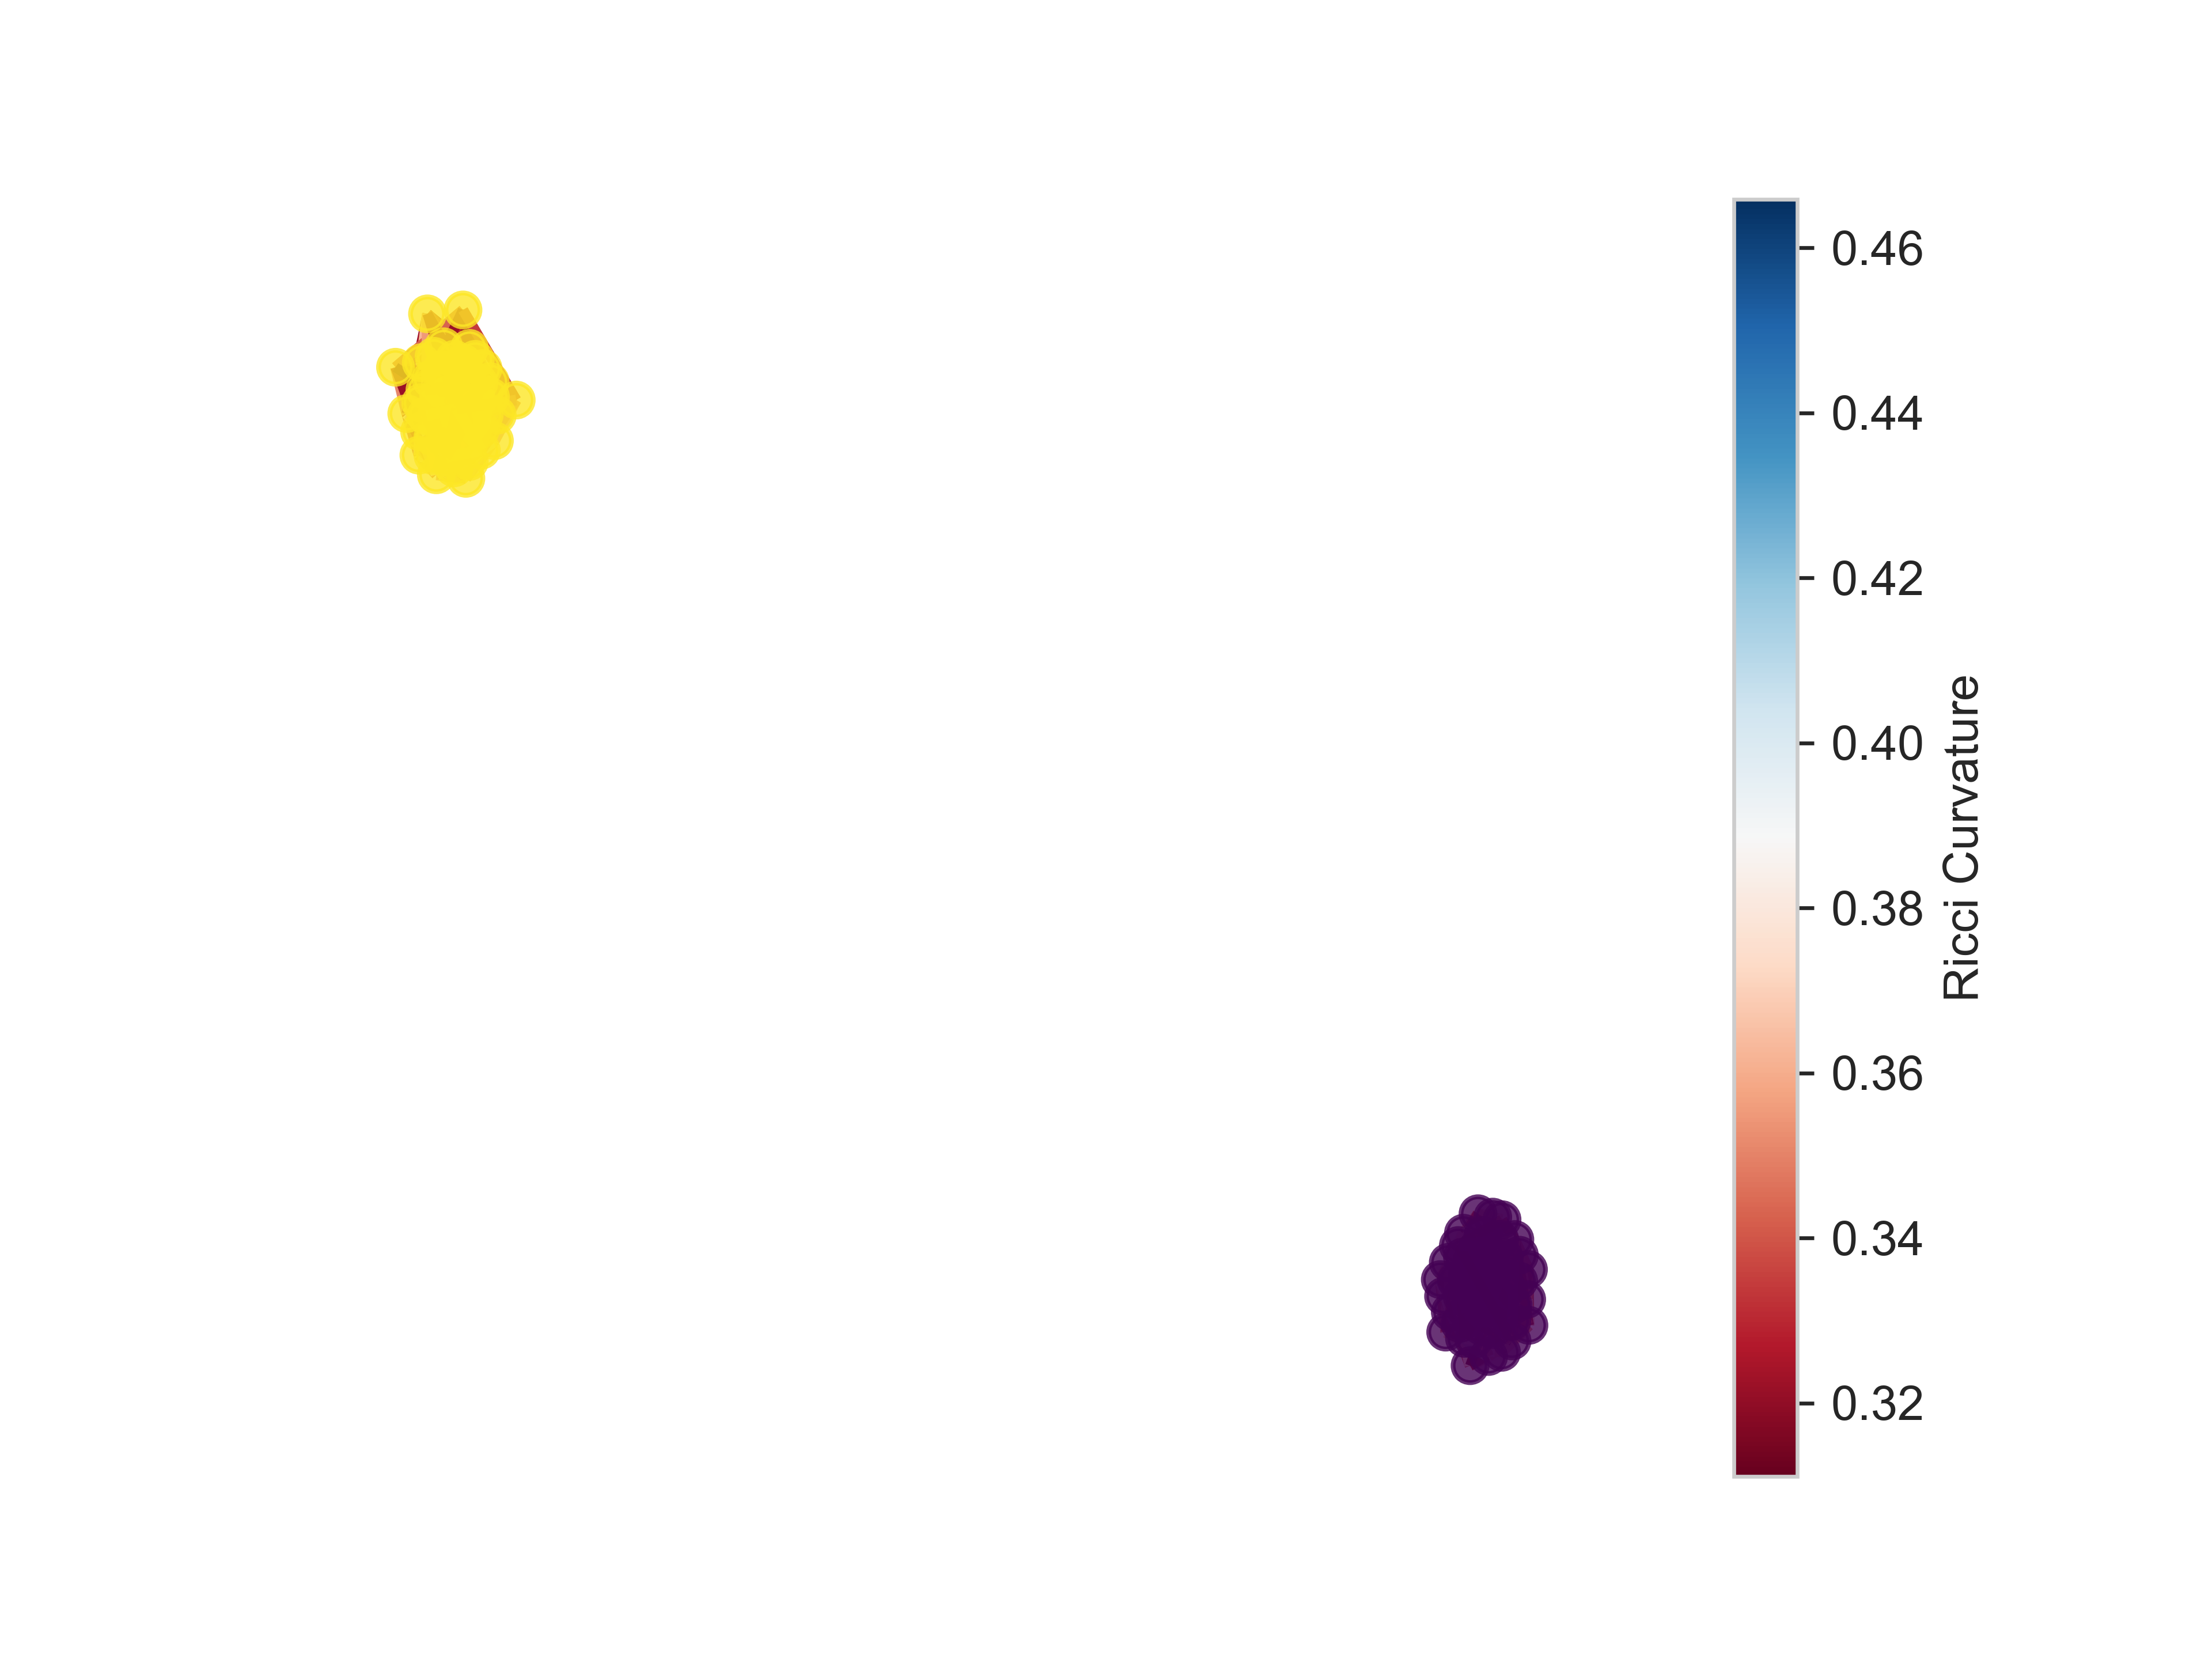
\includegraphics[width=\textwidth]{ToyModelResults/SBM_results/Communities.png}
        \caption{Detected communities.}
        \label{fig:sbm_result}
    \end{subfigure}
    \caption{Comparison of the initial SBM graph and the community detection result.}
    \label{fig2}
\end{figure}

\begin{figure}[ht]
    \centering
    \begin{subfigure}[b]{0.45\textwidth}
        \centering
        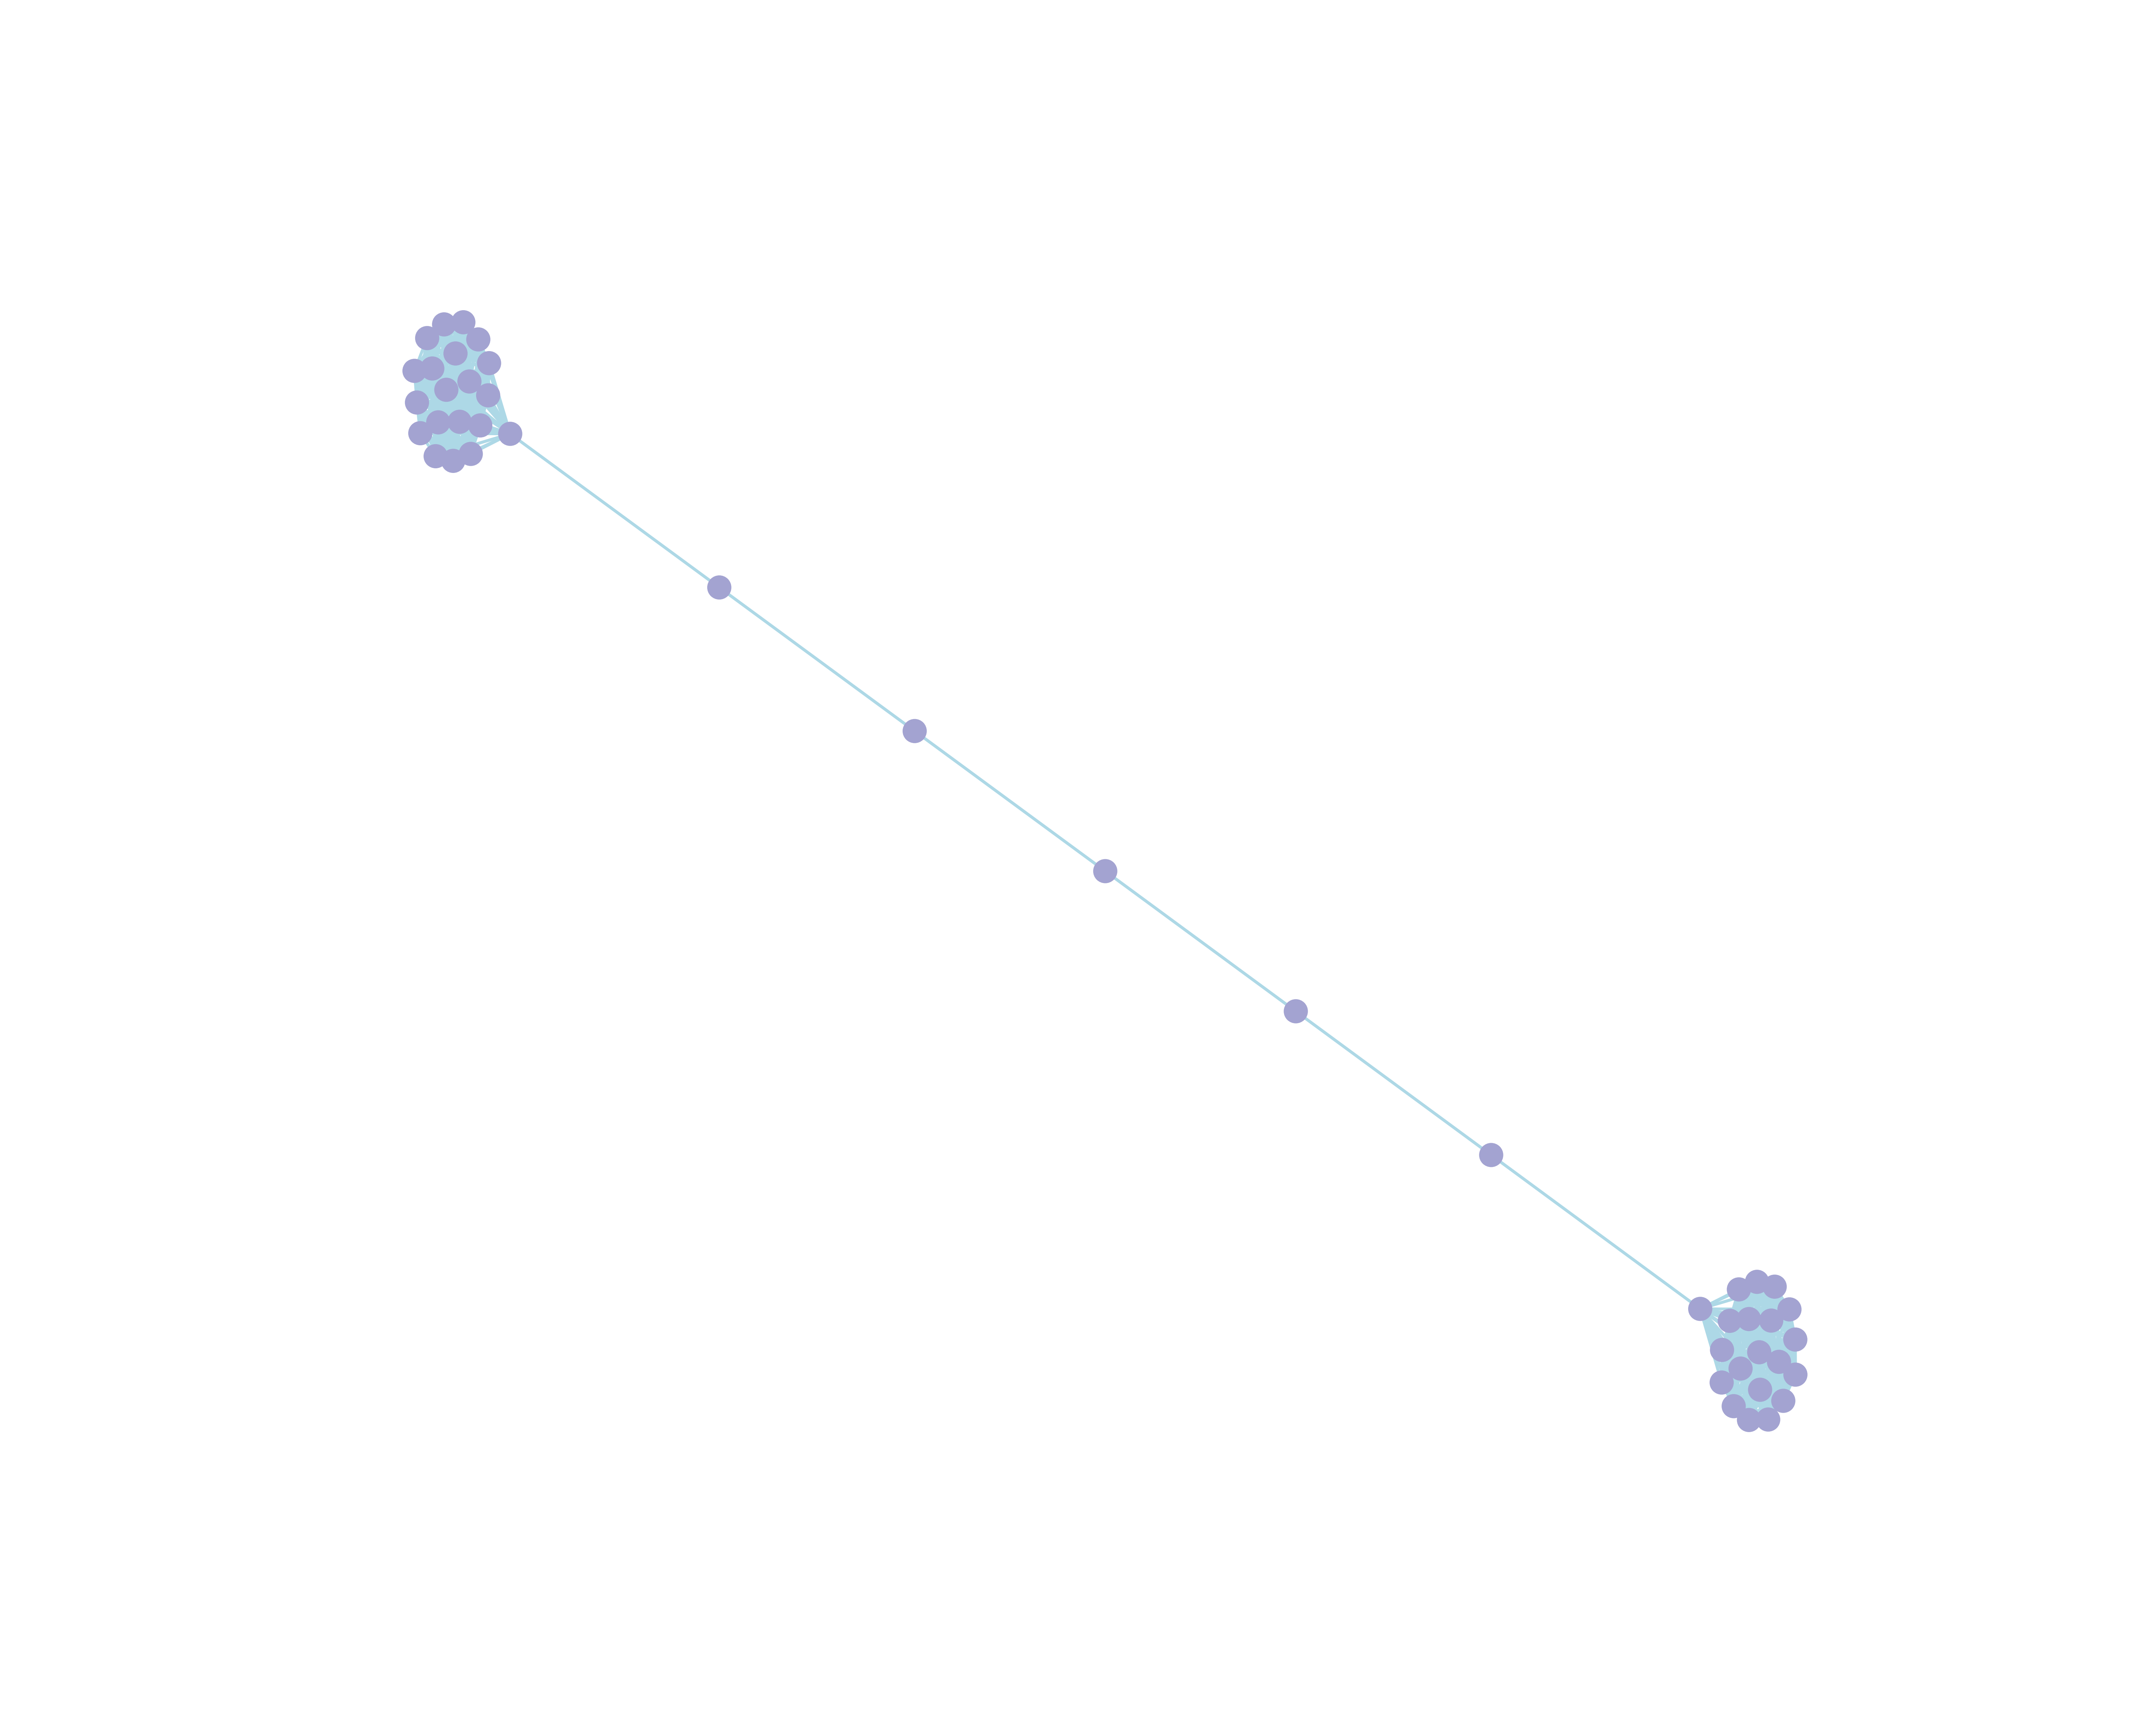
\includegraphics[width=\textwidth]{ToyModelResults/Barbell_resluts/BeforeRicciFlow.png}
        \caption{Initial Barbell graph}
        \label{fig:barbell_initial}
    \end{subfigure}
    \hfill
    \begin{subfigure}[b]{0.45\textwidth}
        \centering
        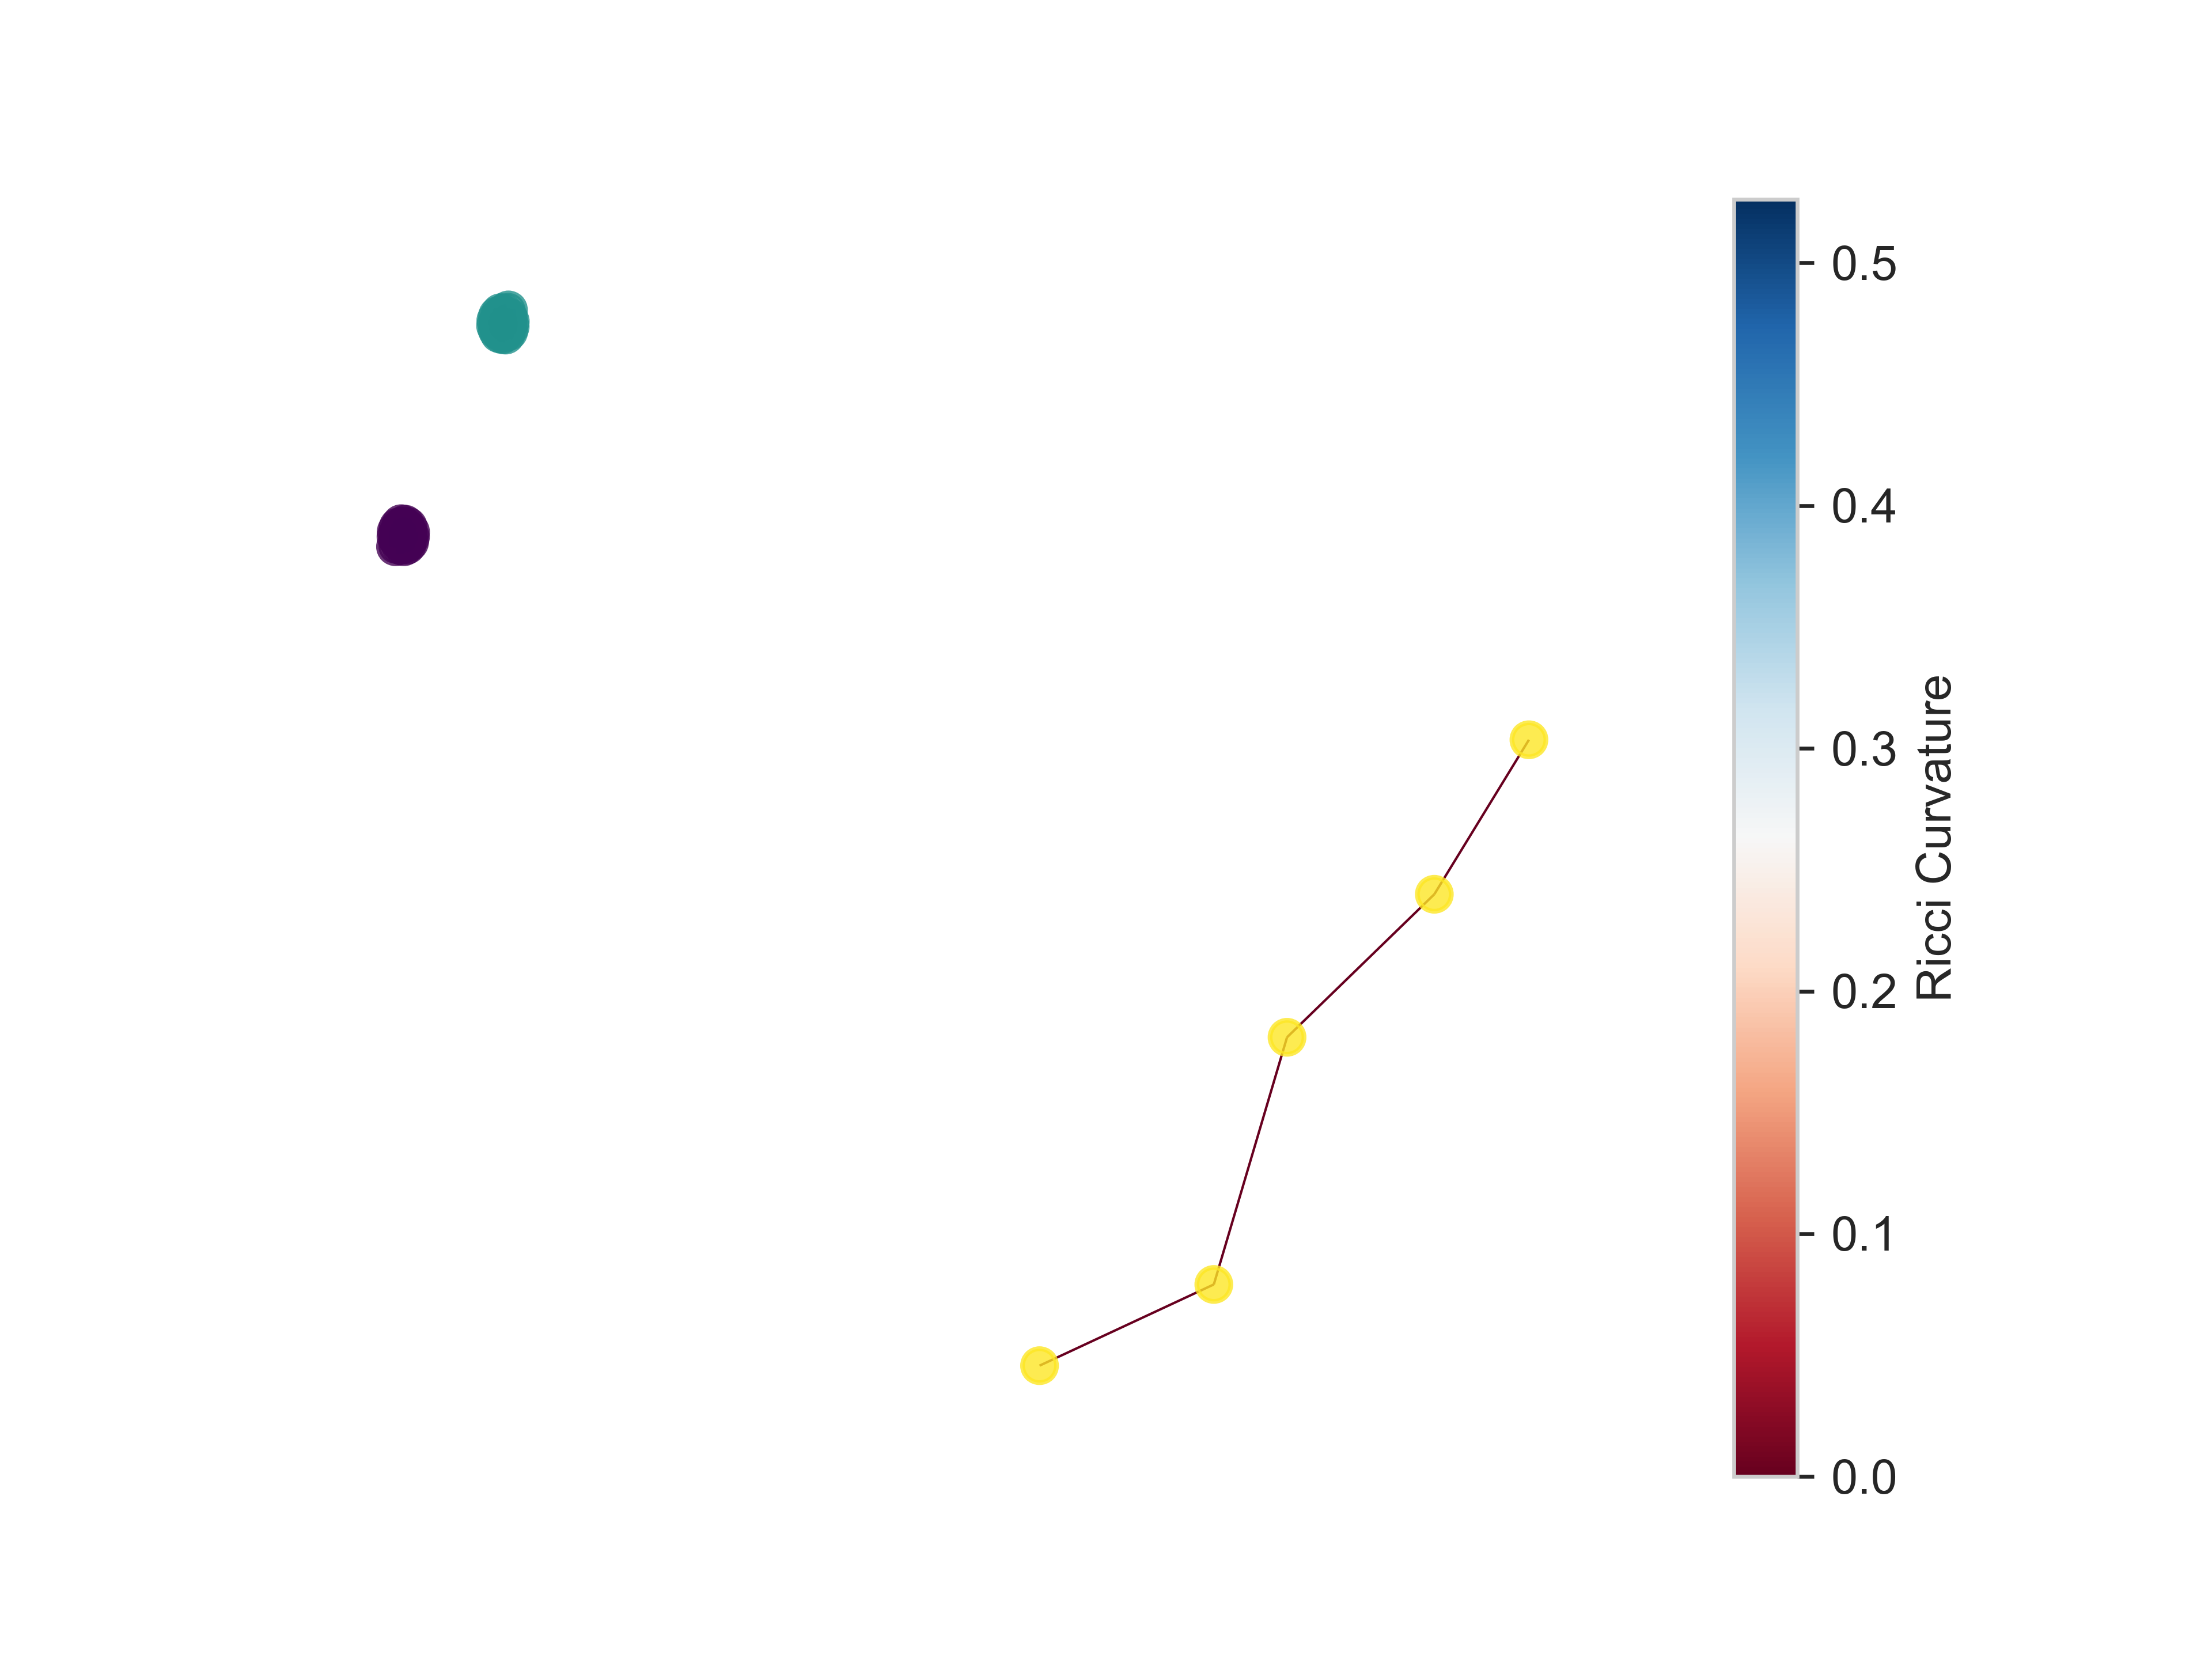
\includegraphics[width=\textwidth]{ToyModelResults/Barbell_resluts/Communities.png}
        \caption{Detected communities}
        \label{fig:barbell_result}
    \end{subfigure}
    \caption{Comparison of the initial Barbell graph and the community detection result.}
    \label{fig3}
\end{figure}

\begin{figure}[ht!]
    \centering
    \begin{subfigure}[b]{0.45\textwidth}
        \centering
        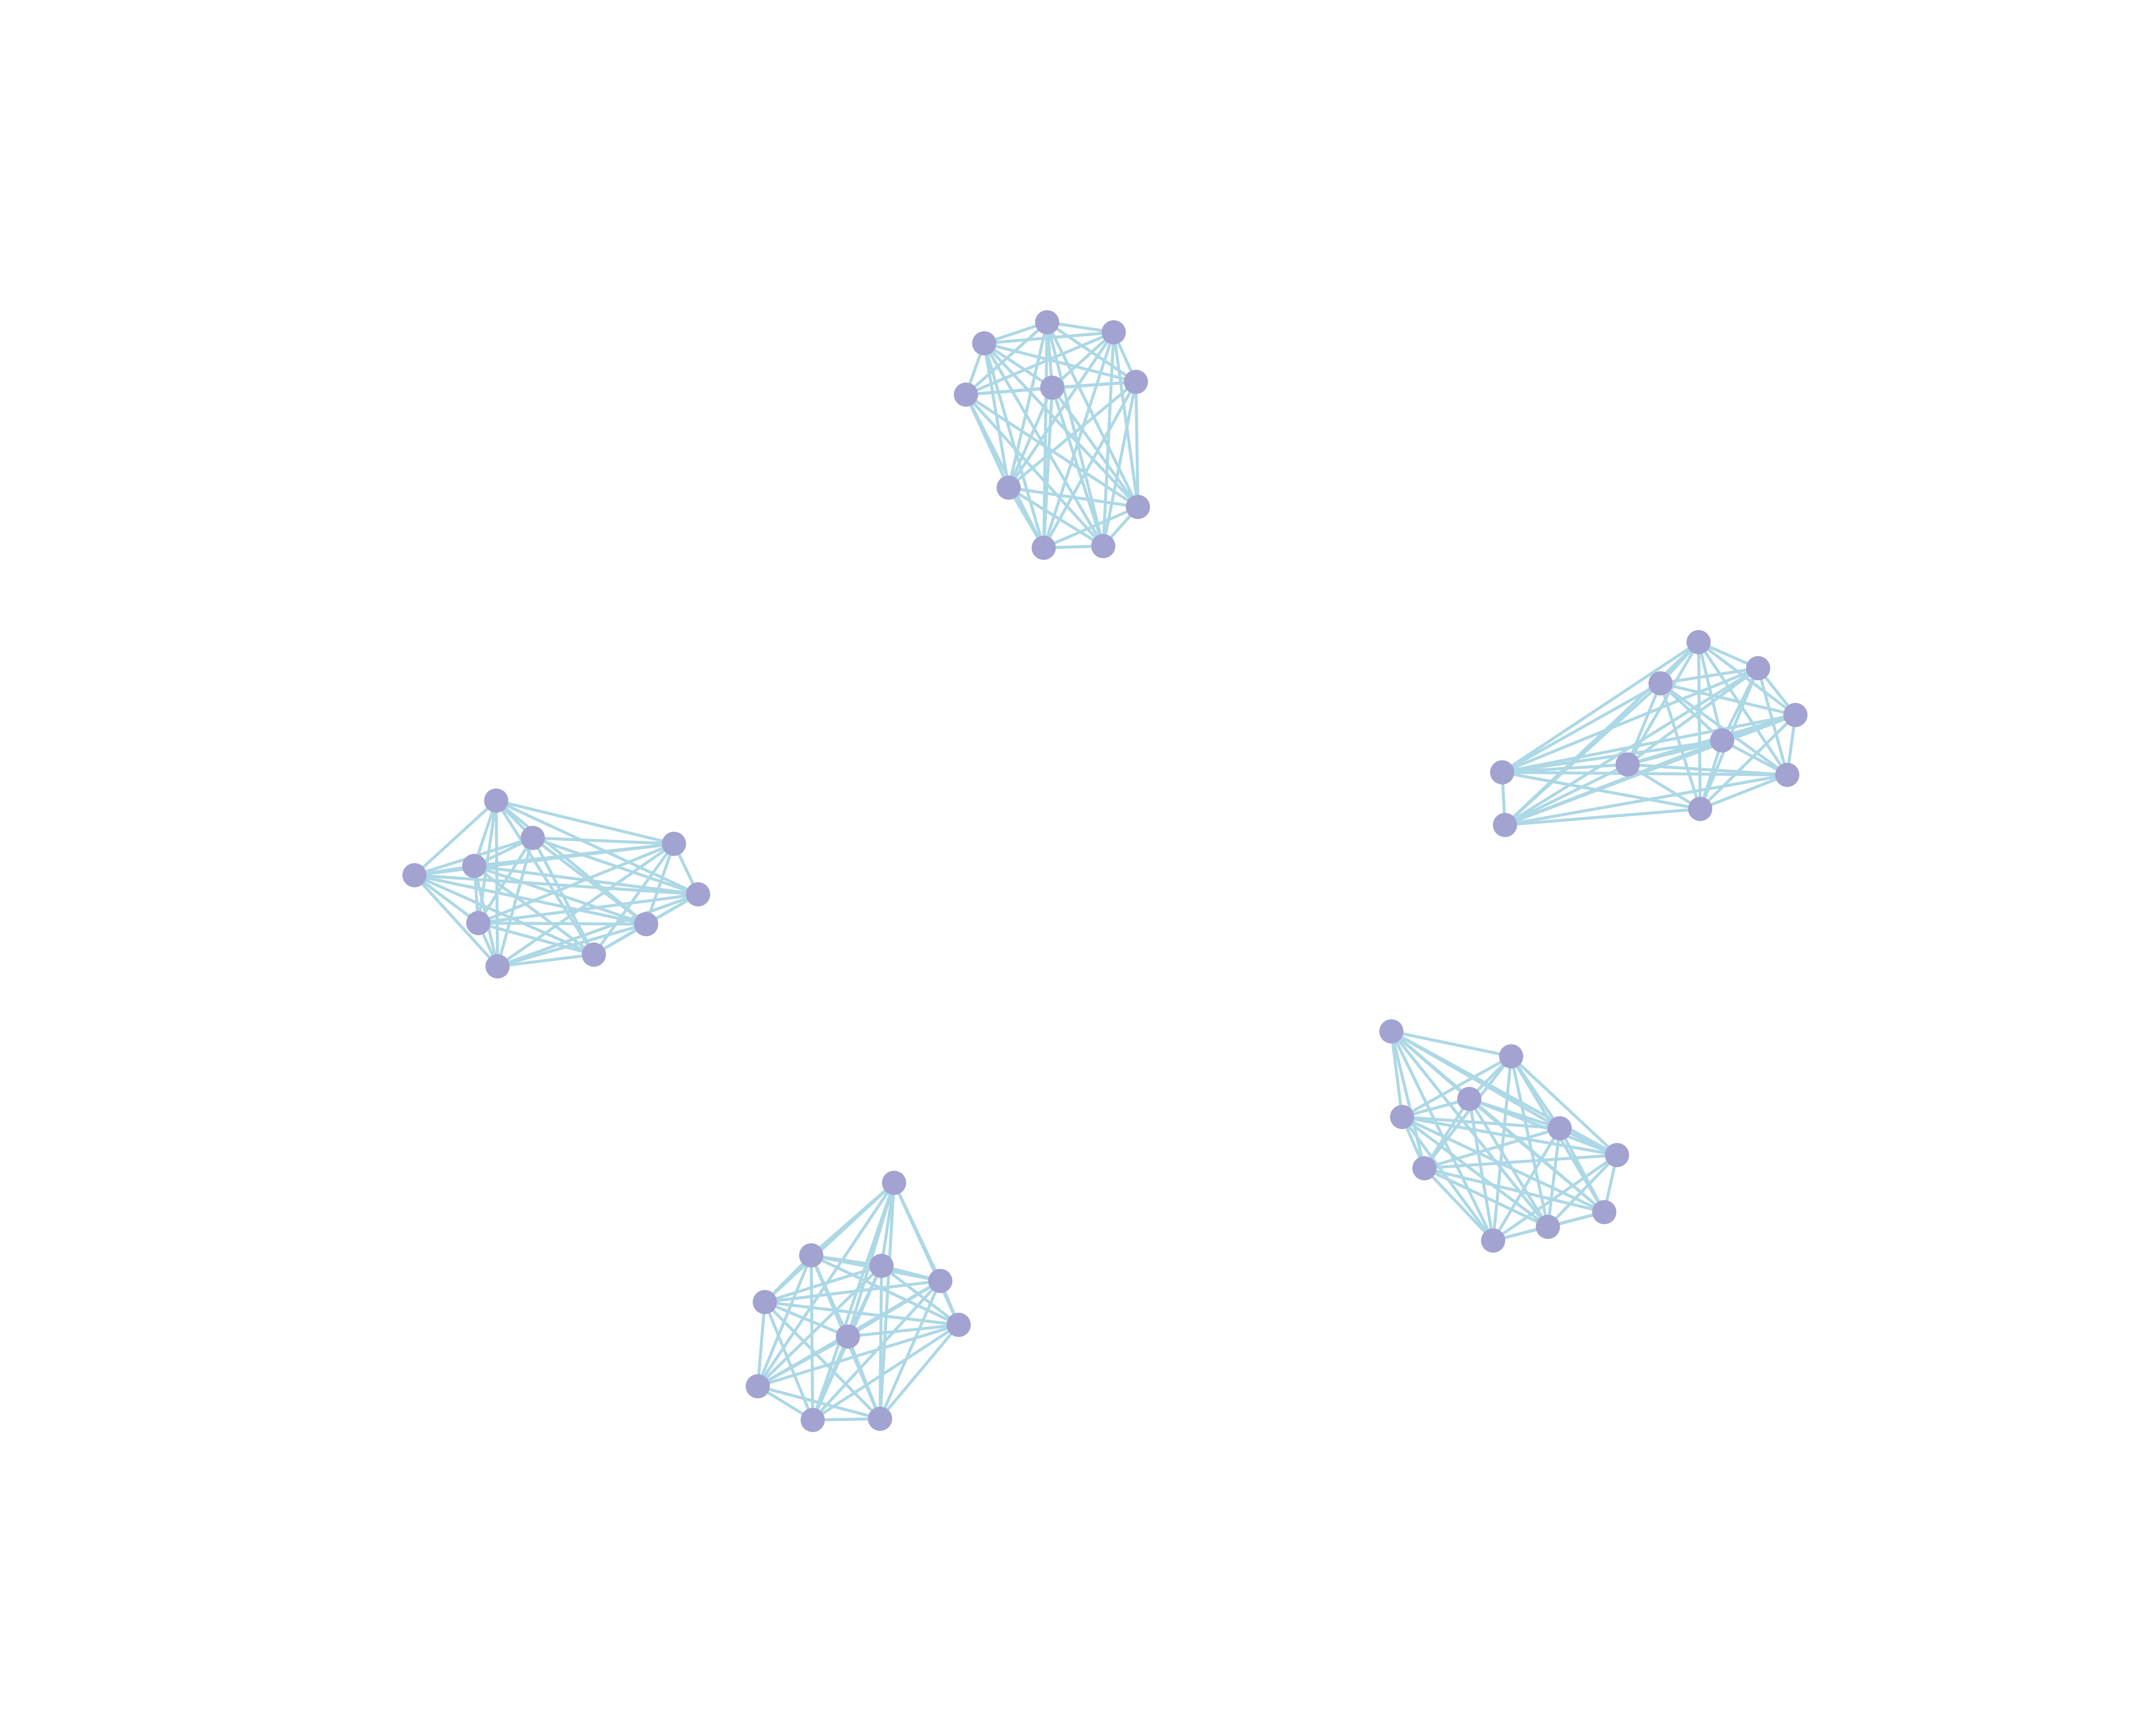
\includegraphics[width=\textwidth]{ToyModelResults/Caveman_resluts/BeforeRicciFlow.png}
        \caption{Initial Caveman graph}
        \label{fig:caveman_initial}
    \end{subfigure}
    \hfill
    \begin{subfigure}[b]{0.45\textwidth}
        \centering
        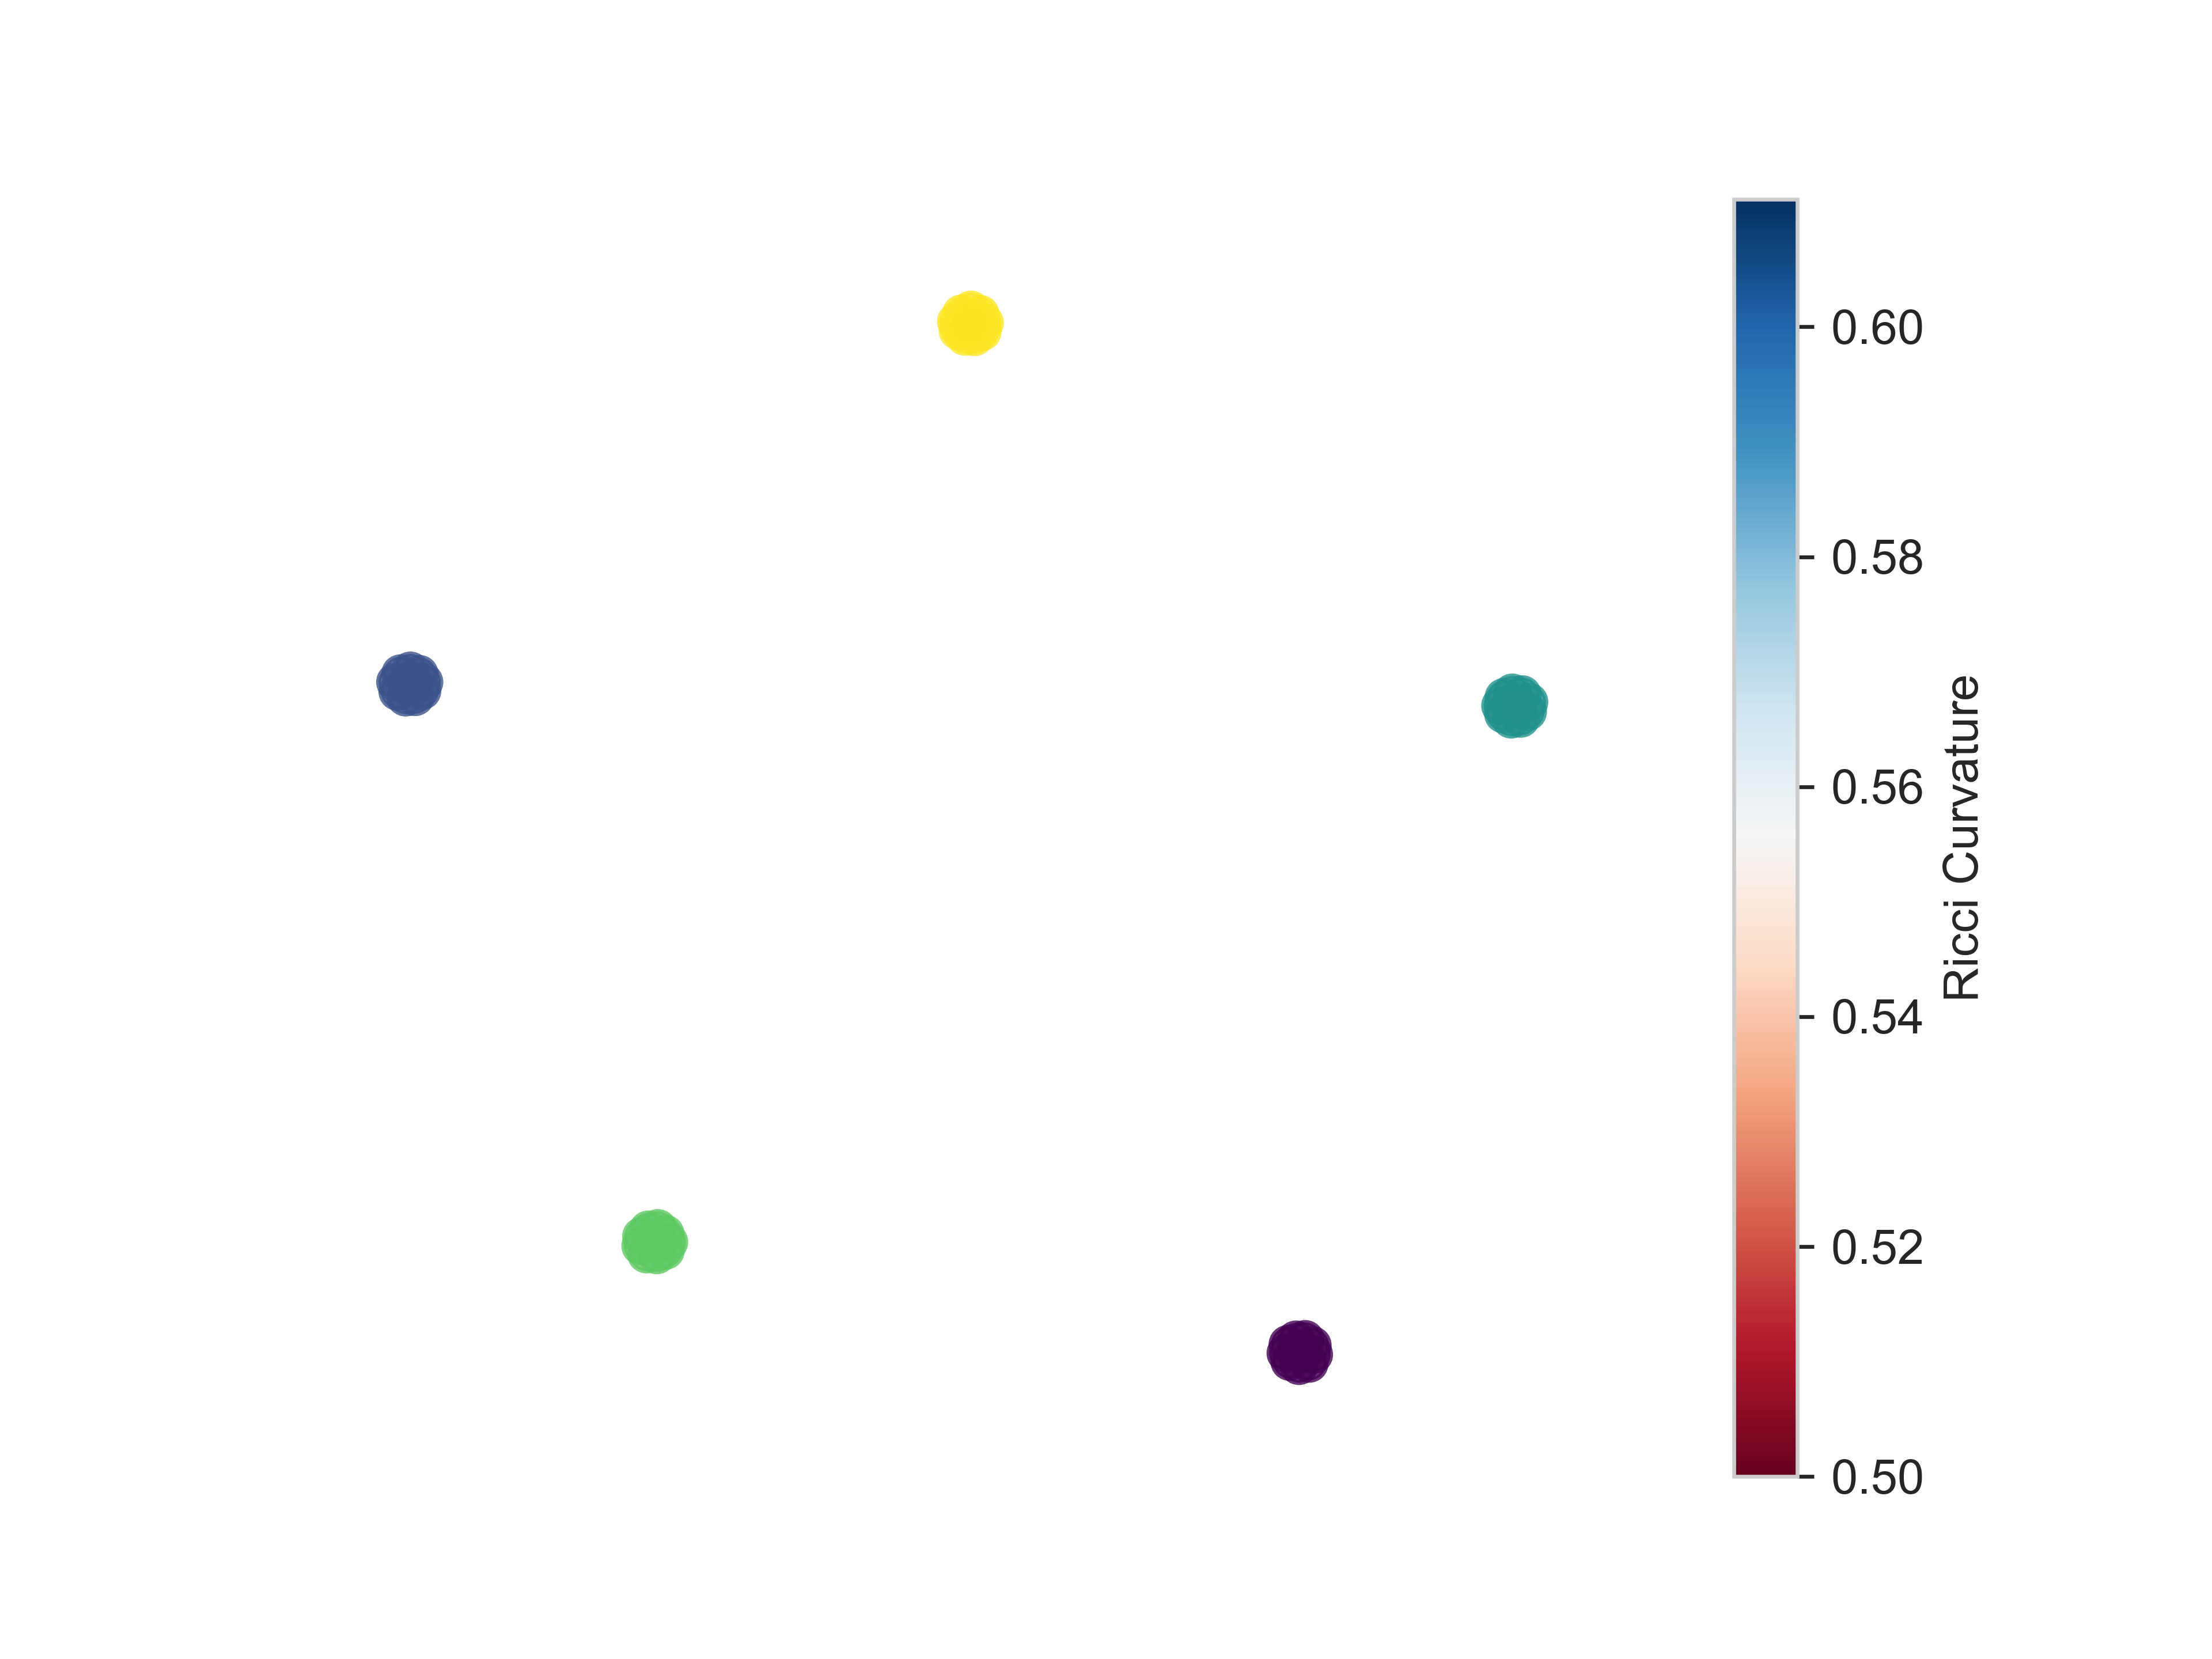
\includegraphics[width=\textwidth]{ToyModelResults/Caveman_resluts/Communities.png}
        \caption{Detected communities}
        \label{fig:caveman_result}
    \end{subfigure}
    \caption{Comparison of the initial Caveman graph and the community detection result.}
    \label{fig4}
\end{figure}


\newpage

\section{Implementation for Planar Graphs}


\subsection{}
\subsection{Results}



%%%% bibliography 
\newpage
\pagestyle{plain}

\setcounter{secnumdepth}{-1}
\printbibliography

\addcontentsline{toc}{section}{\textcolor{black}{References}}

\end{document}